\documentclass[11pt,]{article}
\usepackage{lmodern}
\usepackage{amssymb,amsmath}
\usepackage{ifxetex,ifluatex}
\usepackage{fixltx2e} % provides \textsubscript
\ifnum 0\ifxetex 1\fi\ifluatex 1\fi=0 % if pdftex
  \usepackage[T1]{fontenc}
  \usepackage[utf8]{inputenc}
\else % if luatex or xelatex
  \ifxetex
    \usepackage{mathspec}
  \else
    \usepackage{fontspec}
  \fi
  \defaultfontfeatures{Ligatures=TeX,Scale=MatchLowercase}
\fi
% use upquote if available, for straight quotes in verbatim environments
\IfFileExists{upquote.sty}{\usepackage{upquote}}{}
% use microtype if available
\IfFileExists{microtype.sty}{%
\usepackage{microtype}
\UseMicrotypeSet[protrusion]{basicmath} % disable protrusion for tt fonts
}{}
\usepackage[margin=1in]{geometry}
\usepackage{hyperref}
\hypersetup{unicode=true,
            pdftitle={Modulation of sensory behavior and food choice by an enteric bacteria-produced neurotransmitter},
            pdfauthor={Michael P. O'Donnell\textbackslash{}dagger,\textbackslash{}S, Bennett W. Fox\textbackslash{}ddagger, Pin-Hao Chao\textbackslash{}dagger, Frank C. Schroeder\textbackslash{}ddagger and Piali Sengupta\textbackslash{}dagger,\textbackslash{}S},
            pdfborder={0 0 0},
            breaklinks=true}
\urlstyle{same}  % don't use monospace font for urls
\usepackage{graphicx,grffile}
\makeatletter
\def\maxwidth{\ifdim\Gin@nat@width>\linewidth\linewidth\else\Gin@nat@width\fi}
\def\maxheight{\ifdim\Gin@nat@height>\textheight\textheight\else\Gin@nat@height\fi}
\makeatother
% Scale images if necessary, so that they will not overflow the page
% margins by default, and it is still possible to overwrite the defaults
% using explicit options in \includegraphics[width, height, ...]{}
\setkeys{Gin}{width=\maxwidth,height=\maxheight,keepaspectratio}
\setlength{\emergencystretch}{3em}  % prevent overfull lines
\providecommand{\tightlist}{%
  \setlength{\itemsep}{0pt}\setlength{\parskip}{0pt}}
\setcounter{secnumdepth}{0}
% Redefines (sub)paragraphs to behave more like sections
\ifx\paragraph\undefined\else
\let\oldparagraph\paragraph
\renewcommand{\paragraph}[1]{\oldparagraph{#1}\mbox{}}
\fi
\ifx\subparagraph\undefined\else
\let\oldsubparagraph\subparagraph
\renewcommand{\subparagraph}[1]{\oldsubparagraph{#1}\mbox{}}
\fi

%%% Use protect on footnotes to avoid problems with footnotes in titles
\let\rmarkdownfootnote\footnote%
\def\footnote{\protect\rmarkdownfootnote}

%%% Change title format to be more compact
\usepackage{titling}

% Create subtitle command for use in maketitle
\providecommand{\subtitle}[1]{
  \posttitle{
    \begin{center}\large#1\end{center}
    }
}

\setlength{\droptitle}{-2em}

  \title{Modulation of sensory behavior and food choice by an enteric
bacteria-produced neurotransmitter}
    \pretitle{\vspace{\droptitle}\centering\huge}
  \posttitle{\par}
    \author{Michael P. O'Donnell\textsuperscript{\(\dagger\),\(\S\)}, Bennett W.
Fox\textsuperscript{\(\ddagger\)}, Pin-Hao
Chao\textsuperscript{\(\dagger\)}, Frank C.
Schroeder\textsuperscript{\(\ddagger\)} and Piali
Sengupta\textsuperscript{\(\dagger\),\(\S\)}}
    \preauthor{\centering\large\emph}
  \postauthor{\par}
    \date{}
    \predate{}\postdate{}
  
\newcommand{\bcenter}{\begin{center}}
\newcommand{\ecenter}{\end{center}}
\usepackage{setspace}

\doublespacing
\usepackage{fontspec}
\setmainfont{Georgia}

\begin{document}
\maketitle
\begin{abstract}
\singlespacing Animals coexist in commensal, pathogenic or mutualistic
relationships with complex communities of diverse organisms including
microbes\textsuperscript{1}. Some bacteria produce bioactive
neurotransmitters which have been proposed to modulate host nervous
system activity and behaviors\textsuperscript{2}. However, the
mechanistic basis of this microbiota-brain modulation and its
physiological relevance is largely unknown. Here we show that in
\textit{C. elegans}, the neuromodulator tyramine (TA) produced by
gut-colonizing commensal \textit{Providencia} bacteria can bypass the
requirement for host TA biosynthesis to manipulate a host sensory
decision. Bacterially-produced TA is likely converted to octopamine (OA)
by the host tyramine beta-hydroxylase enzyme. OA, in turn, targets the
OCTR-1 receptor on the ASH/ASI sensory neurons to modulate an aversive
olfactory response. We identify genes required for TA biosynthesis in
\textit{Providencia}, and show that these genes are necessary for
modulation of host behavior. We further find that \textit{C. elegans}
colonized by \textit{Providencia} preferentially select these bacteria
in food choice assays, and that this selection bias requires
bacterially-produced TA. Our results demonstrate that a neurotransmitter
produced by gut microbiota mimics the functions of the cognate host
molecule to override host control of a sensory decision, thereby
promoting fitness of both host and microbe.
\end{abstract}

\begin{center}
\fontsize{8}{8}
\fontseries{b}
\selectfont

\textsuperscript{\(\dagger\)}Department of Biology Brandeis University
Waltham, MA 02454

\textsuperscript{\(\ddagger\)}Boyce Thompson Institute and Department of
Chemistry and Chemical Biology Cornell University Ithaca, NY 14853

\textsuperscript{\(\S\)}Corresponding authors: M.O'D:
\href{mailto:mikeod@brandeis.edu}{\nolinkurl{mikeod@brandeis.edu}}; PS:
\href{mailto:sengupta@brandeis.edu}{\nolinkurl{sengupta@brandeis.edu}}
\vskip 0.2in

\par

\noindent

\rule{\textwidth}{0.4pt}

\fontsize{11}{12}
\fontseries{b}
\selectfont

\vskip 0.2in

\end{center}

The pathways mediating chemical communication between gut-colonizing
bacteria and the host nervous system are largely
undescribed\textsuperscript{2}. Recently, the nematode
\textit{C. elegans} has emerged as a powerful system in which to study
host-microbe chemical communication\textsuperscript{3}, offering an
opportunity to experimentally address how microbiota influence host
nervous system function. Diverse populations of pathogenic and
non-pathogenic bacteria both colonize the \emph{C. elegans} intestine
and serve as its primary food source in the wild\textsuperscript{4}.
Exposure to pathogenic bacteria alters \textit{C. elegans} olfactory
behaviors\textsuperscript{5}, but whether commensal gut bacteria also
modulate host behaviors is unknown\textsuperscript{4}.

To identify novel modes of microbial influences on host sensory
behaviors, we screened non-pathogenic bacterial strains typically
associated with wild nematodes\textsuperscript{6} for their ability to
influence \textit{C. elegans} olfactory responses. In long-range
chemotaxis assays\textsuperscript{7}, adult hermaphrodites co-cultivated
on these bacterial strains exhibited robust attraction to a panel of
attractive volatile odorants similar to the behaviors of animals grown
on the standard \textit{E. coli} food source OP50 (Fig. 1a). However,
co-cultivation with the \textit{Providencia alcalifaciens} strain
(JUb39)\textsuperscript{6,8} resulted in decreased avoidance of 100\%
1-octanol as compared to OP50-grown animals (Fig. 1b; this decreased
avoidance is henceforth referred to as octanol modulation). Avoidance of
the volatile and osmotic repellents 2-nonanone and 8M glycerol,
respectively, was unaffected upon growth on JUb39 (Fig. 1b, Fig. S1a),
suggesting that JUb39 modulates responses of \textit{C. elegans} to a
selective subset of nociceptive chemical stimuli. Animals grown on a
distantly-related \textit{Providencia rettgeri} strain isolated from
nematodes in compost (PYb007, Fig. S1b) exhibited similar octanol
modulation (Fig. 1c). These observations indicate that upon co-culture,
multiple \textit{Providencia} strains modulate octanol aversion in
\textit{C. elegans}.

Under specific conditions, food deprivation reduces octanol
avoidance\textsuperscript{9}. JUb39 has been categorized as a
`beneficial' bacterium that supports robust \textit{C. elegans} growth
and does not induce stress responses\textsuperscript{6}, suggesting that
JUb39-fed animals are unlikely to be nutrition-deprived. In support of
this notion, growth on JUb39 did not alter expression of a
\emph{tph-1p::gfp} fusion gene, a reporter of feeding
state\textsuperscript{10,11} (Fig. S1c). Moreover, growth of
\textit{C. elegans} on the poor bacterial food \emph{Bacillus
megaterium}\textsuperscript{12} did not alter octanol avoidance (Fig.
1b). We infer that the observed octanol modulation by
\textit{Providencia} is unlikely to be solely due to changes in feeding
state.

While OP50 is typically crushed by the pharyngeal grinder in young adult
\textit{C. elegans}\textsuperscript{13}, a subset of bacterial strains
can bypass the grinder and survive in the worm
intestine\textsuperscript{6,14,15}. We found that feeding
\textit{C. elegans} with JUb39 pre-treated with high concentrations of
the antibiotic gentamicin eliminated octanol modulation (Fig. 1d),
indicating that JUb39 must be alive to mediate this behavioral
plasticity. In addition, neither exposure of OP50-grown animals to
JUb39-derived odors nor pre-incubation of OP50-grown animals with
JUb39-conditioned media was sufficient to result in octanol modulation
(Fig. S1d-e), further suggesting that \textit{C. elegans} must ingest
live JUb39 to induce octanol modulation.

To test whether colonization of the worm gut drives octanol modulation,
we transformed OP50 and JUb39 with a plasmid encoding a constitutively
expressed mCherry fluorescent reporter. While the guts of OP50-fed adult
worms displayed only diffuse intestinal fluorescence consistent with
these bacteria being lysed, the guts of JUb39-fed worms contained
variable but typically large numbers of intact rod-shaped cells
expressing mCherry (Fig. 1e), likely indicating the presence of live
JUb39. These cells tended to be enriched in the posterior intestine
(Fig. 1e), unlike the reported localization pattern of severely
pathogenic bacteria\textsuperscript{16}. Moreover, nematodes colonized
by JUb39 did not exhibit phenotypes characteristic of pathogenic
infection such as anal swelling\textsuperscript{17} (Fig. 1e), further
confirming that JUb39 is largely non-pathogenic to \textit{C. elegans}.

\begin{center}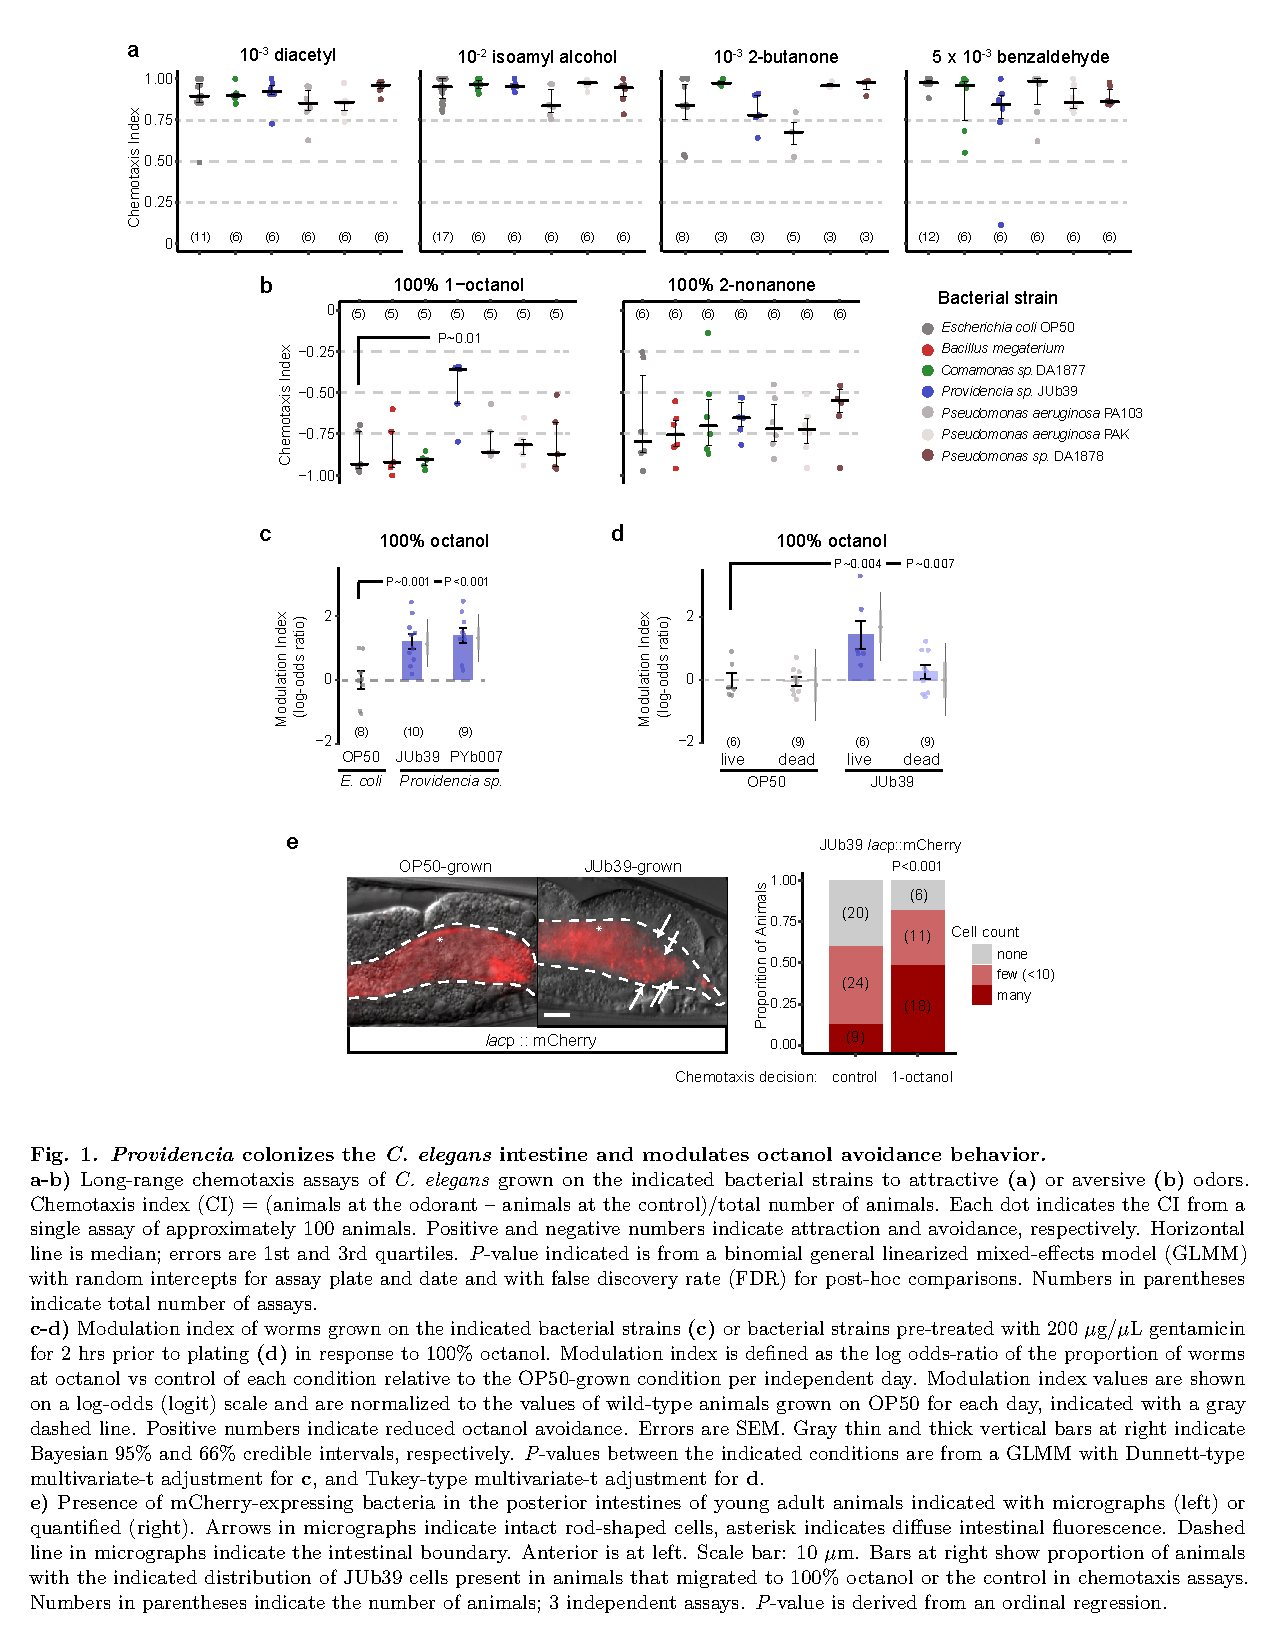
\includegraphics[width=1.05\linewidth]{Figure1} \end{center}

We next performed chemotaxis assays with animals fed on mCherry-labeled
JUb39, and quantified intestinal bacterial cells in animals that had
navigated either toward octanol or toward the control. We found that
animals navigating toward octanol consistently contained more gut
bacteria (Fig. 1e). We conclude that JUb39 colonizes the worm gut and
the extent of colonization is correlated with decision-making in
response to octanol.

We investigated the mechanistic basis for \textit{Providencia}-mediated
octanol modulation. Octanol avoidance is subject to extensive modulation
directly and indirectly via multiple biogenic amines including tyramine
(TA) and octopamine (OA) (Fig. 2a) as well as
neuropeptides\textsuperscript{9,18-22}. TA is produced from Tyrosine
(L-Tyr) via the activity of a tyrosine decarboxylase (TDC; encoded by
\emph{tdc-1} in \textit{C. elegans}); TA is subsequently converted to OA
via a tyramine beta hydroxylase (encoded by
\emph{tbh-1})\textsuperscript{23} (Fig. 2a). Consequently, all
\emph{tbh-1} mutant phenotypes resulting from lack of OA are expected to
be shared by \emph{tdc-1} mutants\textsuperscript{23}. Unexpectedly, we
found that while \emph{tdc-1} mutants grown on JUb39 continued to
exhibit octanol modulation, the modulation exhibited by \emph{tbh-1}
mutants was significantly reduced (Fig. 2b). Mutations in the
\emph{cat-2} tyrosine hydroxylase\textsuperscript{24} and \emph{tph-1}
tryptophan hydroxylase\textsuperscript{25} enzymes required for the
production of biogenic amines dopamine and serotonin in
\textit{C. elegans}, respectively, did not affect octanol modulation
(Fig. 2b). These results raise the possibility that
\textit{C. elegans}-produced OA, but not TA, is partly necessary for
JUb39-mediated octanol modulation.

To account for these observations, we hypothesized that JUb39 may
produce TA that functionally compensates for the host \emph{tdc-1}
mutation. \emph{tdc-1} mutants grown on OP50 have been reported to
display more rapid aversive responses to dilute (30\%)
octanol\textsuperscript{18}. Exogenous TA suppresses this increased
aversion of \emph{tdc-1} animals but does not alter wild-type responses
under the same conditions\textsuperscript{18}. To test if JUb39 is able
to suppress behavioral defects of \emph{tdc-1} mutants, we performed
short-range acute avoidance assays {[}the ``smell-on-a-stick'' (SOS)
assay{]}\textsuperscript{9,26}. In this assay, the strength of avoidance
is inversely correlated with reversal latency when the animal encounters
the repellent as it is moving forward. As expected, \emph{tdc-1} mutants
grown on OP50 responded more rapidly to 30\% octanol than wild-type
animals (Fig. 2c). This enhanced aversion was suppressed upon growth on
JUb39 (Fig. 2c). These results are consistent with the notion that
bacterially-produced TA functionally complements for the loss of
host-derived TA in driving a sensory behavioral decision.

To directly test for the production of TA by JUb39, we measured
succinyl-TA levels using high-resolution HPLC-MS in wild-type and
\emph{tdc-1} worms grown on either OP50 or JUb39\textsuperscript{27}.
Levels of succinyl-TA were comparable in wild-type animals grown on
either OP50 or JUb39, whereas \emph{tdc-1} mutants grown on OP50 had no
detectable succinyl-TA, consistent with previous
reports\textsuperscript{23} (Fig. 2d, Fig. S2). Notably, succinyl-TA
levels were \linebreak

\begin{center}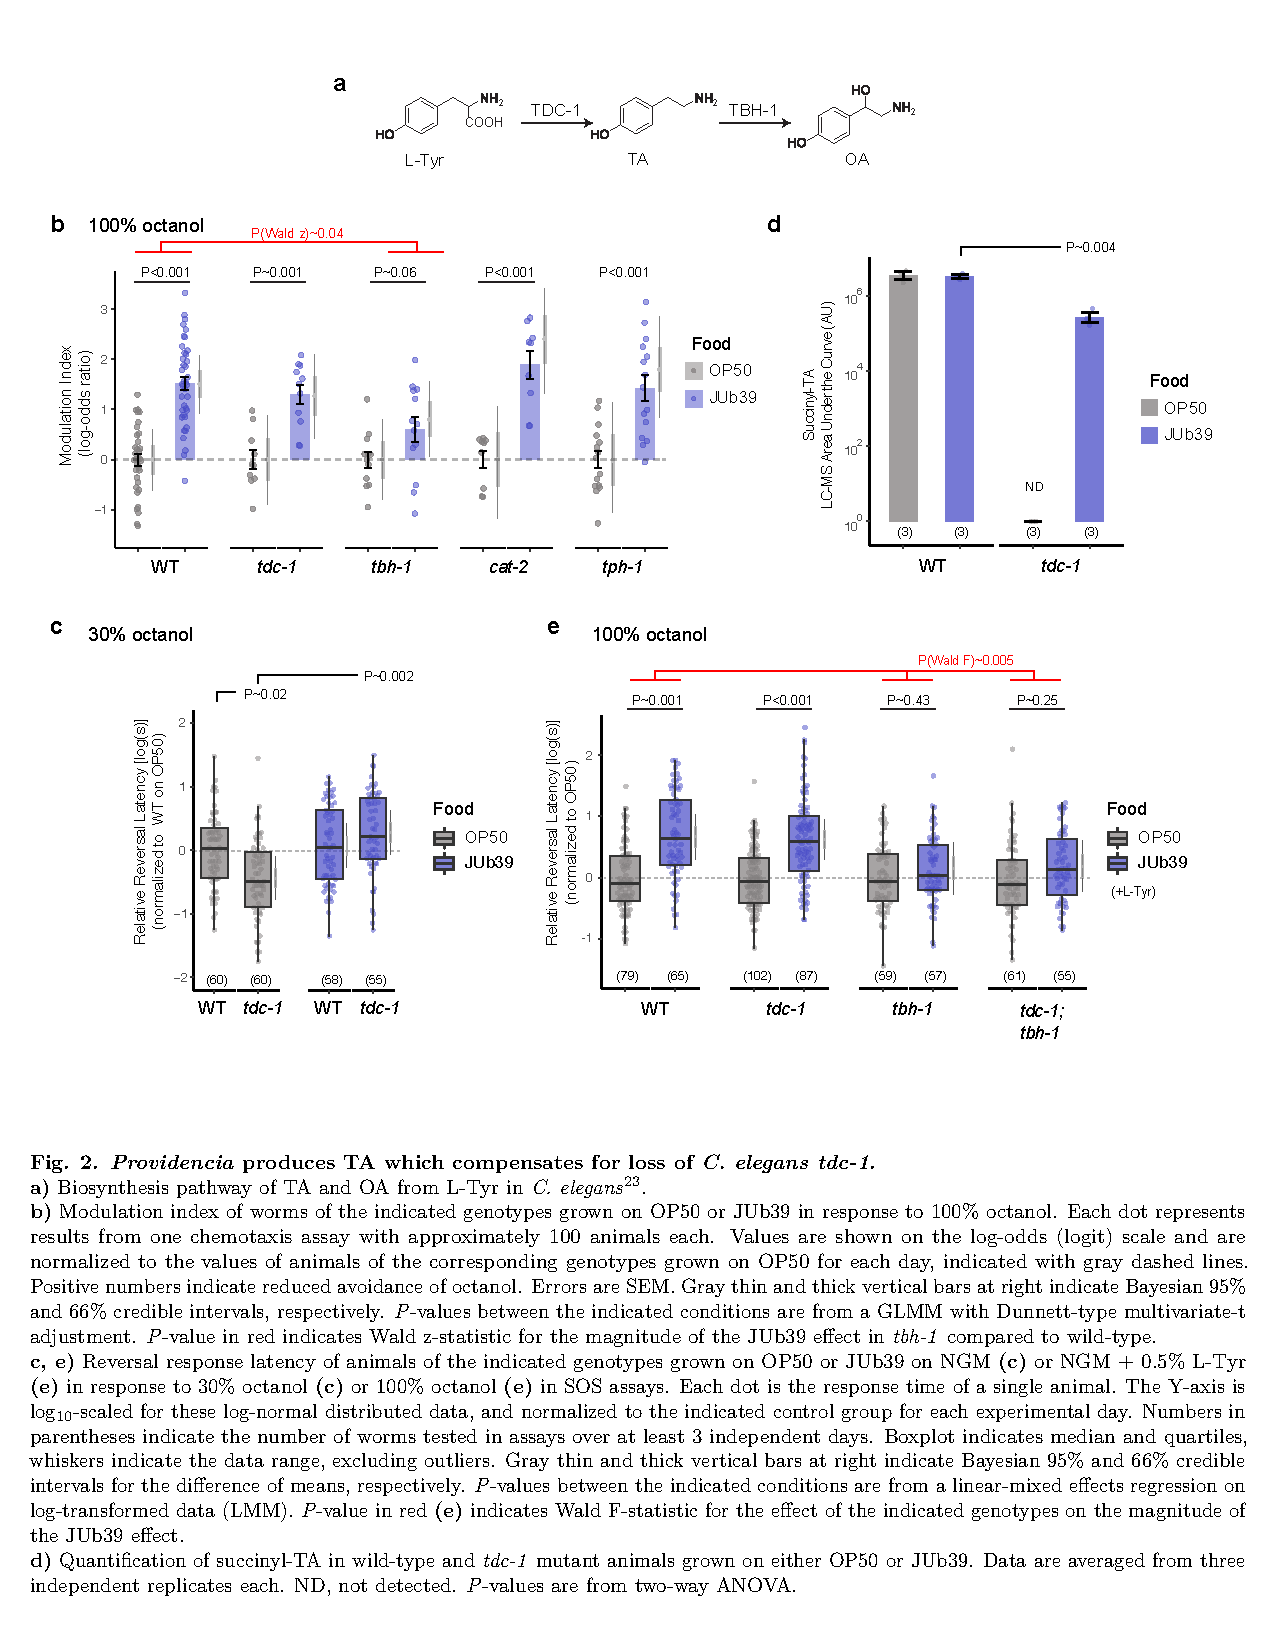
\includegraphics[width=1\linewidth]{Figure2} \end{center}

\noindent partly restored in \emph{tdc-1} mutants grown on JUb39 (Fig.
2d). OA was not detected under these conditions in either wild type or
\emph{tdc-1} mutants. We conclude that JUb39 in association with
\emph{C. elegans} produces TA which can accumulate in the host.

Although TA biosynthesis in bacteria has been demonstrated in some
gram-positive genera, production appears to be uncommon in gram-negative
bacteria which include \emph{Providencia}\textsuperscript{28,29}. TA
production in gram-positive strains is induced upon supplementation with
L-Tyr\textsuperscript{30}. We found that growth on L-Tyr-supplemented
media enhanced octanol modulation by JUb39 in SOS assays (Fig. S3).
Under these conditions, mutations in \emph{tbh-1} fully suppressed
octanol modulation in SOS assays, whereas consistent with our
observations in long-range chemotaxis assays, \emph{tdc-1} mutants
continued to exhibit robust octanol modulation (Fig. 2e). Octanol
avoidance behaviors of \emph{tdc-1; tbh-1} double mutants were similar
to those of \emph{tbh-1} mutants alone (Fig. 2e), indicating that the
lack of host-derived OA, and not accumulation of TA due to loss of
TBH-1\textsuperscript{23,27} accounts for the reduced octanol modulation
in \emph{tbh-1} mutants.

Biogenic amines are typically generated from aromatic amino acids and
L-glutamate by pyridoxyl phosphate (PLP)-dependent group II aromatic
amino acid decarboxylase enzymes (AADCs) in both eukaryotes and
bacteria\textsuperscript{31} (Fig. S4a-b, Table S1). In gram-positive
\emph{Enterococcus} and \emph{Lactobacillus} (\emph{Lb}), TA production
is mediated by the TDC-encoding (\emph{tyrDC}) AADC and tyrosine
permease/transporter (\emph{tyrP}) genes present in an operon; this
operon is inducible by L-Tyr (Fig. 3a-b, S4a-b, Table
S1)\textsuperscript{32,33}. Although genes related to
\emph{Enterococcus} \emph{tyrDC} and \emph{tyrP} were largely absent in
\emph{Gammaproteobacteria} (Fig. 3b), we confirmed the presence of
homologous operons containing \emph{tyrDC} and \emph{tyrP} in JUb39 and
PYb007 in \emph{de novo} genome assemblies via whole genome sequencing
(Fig. 3a, Fig. S4b, Table S1). \emph{tyrDC} homologs were also
identified in the genomes of additional members of the
\emph{Morganellaceae} family, although the operon structure was
conserved in only a subset of these genomes (Fig. 3a, Fig. 3c, S4b,
Table S1).

\emph{Providencia} TyrDC is highly homologous to the \emph{Lb} enzyme,
which has been well characterized with respect to substrate
specificity\textsuperscript{34}. Protein modeling using the crystal
structure of \emph{Lb}-TyrDC\textsuperscript{34} as a guide (see
Methods) indicated that JUb39 TyrDC shares most known catalytic sites
with \emph{Lb}-TyrDC (Fig. 3d). Interestingly, JUb39 TyrDC contains a
substitution at A600 (S586 in \emph{Lb}-TyrDC; Fig.3d), a variant
demonstrated to enhance specific catalytic activity of \emph{Lb}-TyrDC
for tyrosine\textsuperscript{34}. We infer that JUb39 TyrDC likely
generates TA from tyrosine.

\begin{flushleft}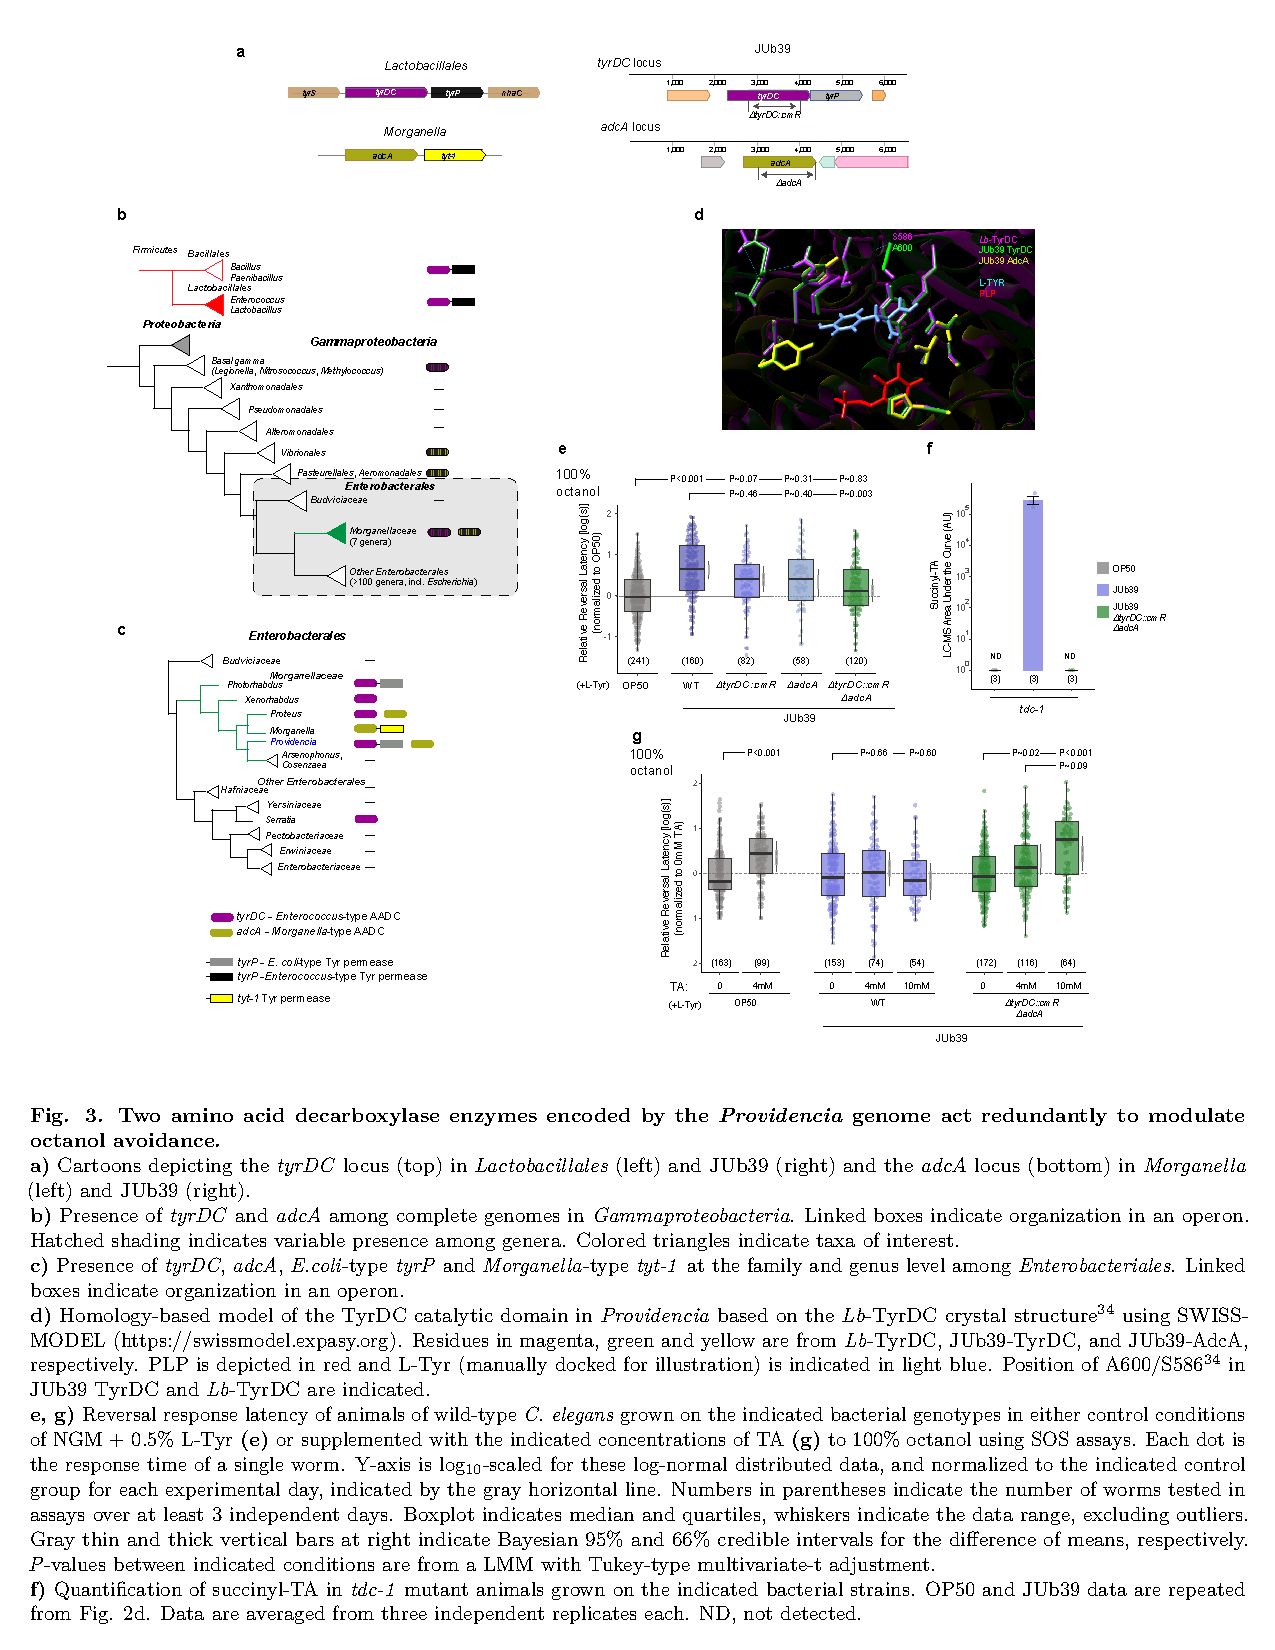
\includegraphics[width=1.1\linewidth]{Figure3} \end{flushleft}

\emph{Morganella} strains (\emph{Morganellaceae} family) have been
reported to produce TA under certain conditions\textsuperscript{28},
despite having no discernible tyrDC orthologs (Fig. 3c, Fig. S4a-b,
Table S1). Instead in \emph{Morganella}, we identified an AADC-encoding
gene (hereafter \emph{adcA}) with \textasciitilde{}29\% and 27\%
sequence identity to \emph{Enterococcus} TyrDC and human GAD67,
respectively, in an operon upstream of a gene encoding a TYT-1 family
tyrosine permease (Fig. 3a, Fig. 3c). An \emph{adcA} homolog is also
present in \emph{Providencia} genomes including in JUb39 but is not
adjacent to a tyrosine transporter (Fig. 3a, Fig. S4a-b, Table S1). We
conclude that \emph{Providencia} encodes at least two AADCs with the
potential to generate TA, and the phylogenetic incongruence suggests
that both tyrDC and \emph{adcA} genes may have either been lost or
acquired in the \emph{Morganellaceae} family via horizontal gene
transfer.

To test whether one or both JUb39 AADCs are necessary for octanol
modulation, we engineered deletions in JUb39 \emph{tyrDC} and
\emph{adcA} (\emph{\(\Delta\)tyrDC::cmR} and \emph{\(\Delta\)adcA},
respectively; Fig. 3a). While cultivation on each deletion-containing
bacterial strain alone weakly decreased octanol modulation, growth on
the JUb39 \emph{\(\Delta\)tyrDC::cmR} \emph{\(\Delta\)adcA} double
knockout bacteria abolished octanol modulation (Fig. 3e). We confirmed
that JUb39 \emph{\(\Delta\)tyrDC::cmR} \emph{\(\Delta\)adcA} colonizes
the \emph{C. elegans} gut (Fig. S5), and further showed that
\emph{tdc-1} animals grown on JUb39 \emph{\(\Delta\)tyrDC::cmR}
\emph{\(\Delta\)adcA} do not produce succinyl-TA (Fig. 3f). Octanol
modulation was restored in wild-type \emph{C. elegans} grown on JUb39
\emph{\(\Delta\)tyrDC::cmR} \emph{\(\Delta\)adcA} strains upon
supplementation with TA (Fig. 3g). Moreover, while exogenous TA did not
further increase octanol avoidance in wild-type JUb39-grown animals, TA
supplementation was sufficient to induce octanol modulation in
OP50-grown animals (Fig. 3g). Together, these results indicate that TA
produced by multiple AADC enzymes in \emph{Providencia} is both
necessary and sufficient to modulate octanol avoidance by wild-type
\emph{C. elegans}.

We next identified the molecular targets of
\textit{Providencia}-mediated octanol modulation in the host. As
bacterially-produced TA is likely converted to OA via the host TBH-1
enzyme\textsuperscript{23} to mediate octanol modulation, we focused
primarily on host OA receptors. The bilateral ASH nociceptive neurons
located in the head amphid organs of \textit{C. elegans} have been
implicated in sensing octanol\textsuperscript{9,19,26}. These neurons
express multiple TA and OA receptors, a subset of which is required for
octanol modulation by these monoamines\textsuperscript{18,35}. Among
ASH-expressed OA receptors, mutations in \emph{octr-1}, but not
\emph{ser-3}, abolished JUb39-mediated octanol modulation, without
altering the extent of gut colonization (Fig. 4a, Fig. S5). We also
observed an effect on octanol modulation in \emph{tyra-2} TA receptor
mutants, primarily due to decreased octanol avoidance upon growth on
OP50 (4.3 ± 0.25s for \emph{tyra-2} vs.~2.9 ± 0.13s for WT). TYRA-2 has
recently been shown to mediate responses to an OA-linked
pheromone\textsuperscript{36}, although the reason for the observed
effect in OP50-grown animals is currently unclear. Expression of
\emph{octr-1} cDNA in the ASH/ASI sensory neurons restored octanol
modulation (Fig. 4a). \emph{octr-1} mutants also lacked octanol
modulation when grown on JUb39 \emph{\(\Delta\)tyrDC::cmR}
\(\Delta\)\textit{adcA} supplemented with TA (Fig. 4b). We conclude that
host OA produced upon JUb39 colonization acts via OCTR-1 in ASH/ASI to
modulate octanol avoidance.

Next we investigated the biological relevance of the JUb39-directed
decrease in octanol aversion by \textit{C. elegans}. While many
gram-negative enteric bacteria produce long-chain alcohols including
octanol\textsuperscript{37}, whether \textit{Providencia} produces this
chemical is unknown. However, JUb39 and other \textit{Providencia}
strains can produce the branched alcohol isoamyl alcohol (IAA), which is
aversive to \textit{C. elegans} when
concentrated\textsuperscript{38,39}. Similar to octanol, avoidance of
high IAA concentrations is also mediated by the ASH sensory
neurons\textsuperscript{39}. We hypothesized that reduced avoidance of
JUb39-produced aversive alcohols or other odorants may preferentially
bias JUb39-grown \textit{C. elegans} to select these bacteria in food
choice assays. Indeed, animals grown on JUb39 more strongly preferred
JUb39 compared to OP50-grown worms, which showed a slight preference for
JUb39 in a short-range food choice assay (Fig. 4c). The bias towards
JUb39 was eliminated in animals grown on JUb39
\(\Delta\)\textit{tyrDC}::cmR \(\Delta\)\textit{adcA}, suggesting that
bacterial TA production is necessary for this food preference (Fig 4b).
Together, these results imply that TA produced by JUb39 reduces
ASH/ASI-mediated avoidance of JUb39-produced aversive cues such as
concentrated alcohols, to allow preferential selection of these
bacteria.

Our observations support a model in which the neurotransmitter TA
produced by intestinal \emph{Providencia} bacteria modulates aversive
responses of \emph{C. elegans} to the enteric bacteria-produced volatile
metabolite octanol, likely via subverting host-dependent TA production.
Bacterially-produced TA is converted to OA by \emph{C. elegans} TBH-1;
OA subsequently acts on the ASH/ASI neurons via the OCTR-1 OA receptor
to decrease aversion of octanol. Bacterially-derived TA also increases
the preference of \emph{C. elegans} for \emph{Providencia} in food
choice assays (Fig. 4d). We speculate that the preference for
\emph{Providencia} upon colonization of \emph{C. elegans} by these
bacteria promotes increased consumption leading to stable
association\textsuperscript{4,40} and bacterial dispersal. As
\emph{Providencia} is a rich food source for \emph{C.
elegans}\textsuperscript{6}, this association may be mutually
beneficial. Our results describe a pathway by which neurotransmitters
produced by commensal bacterial direct host behavioral decisions by
supplementing or compensating for the activity of key host biosynthetic
enzymes, thereby altering fitness of both host and microbe.

\begin{center}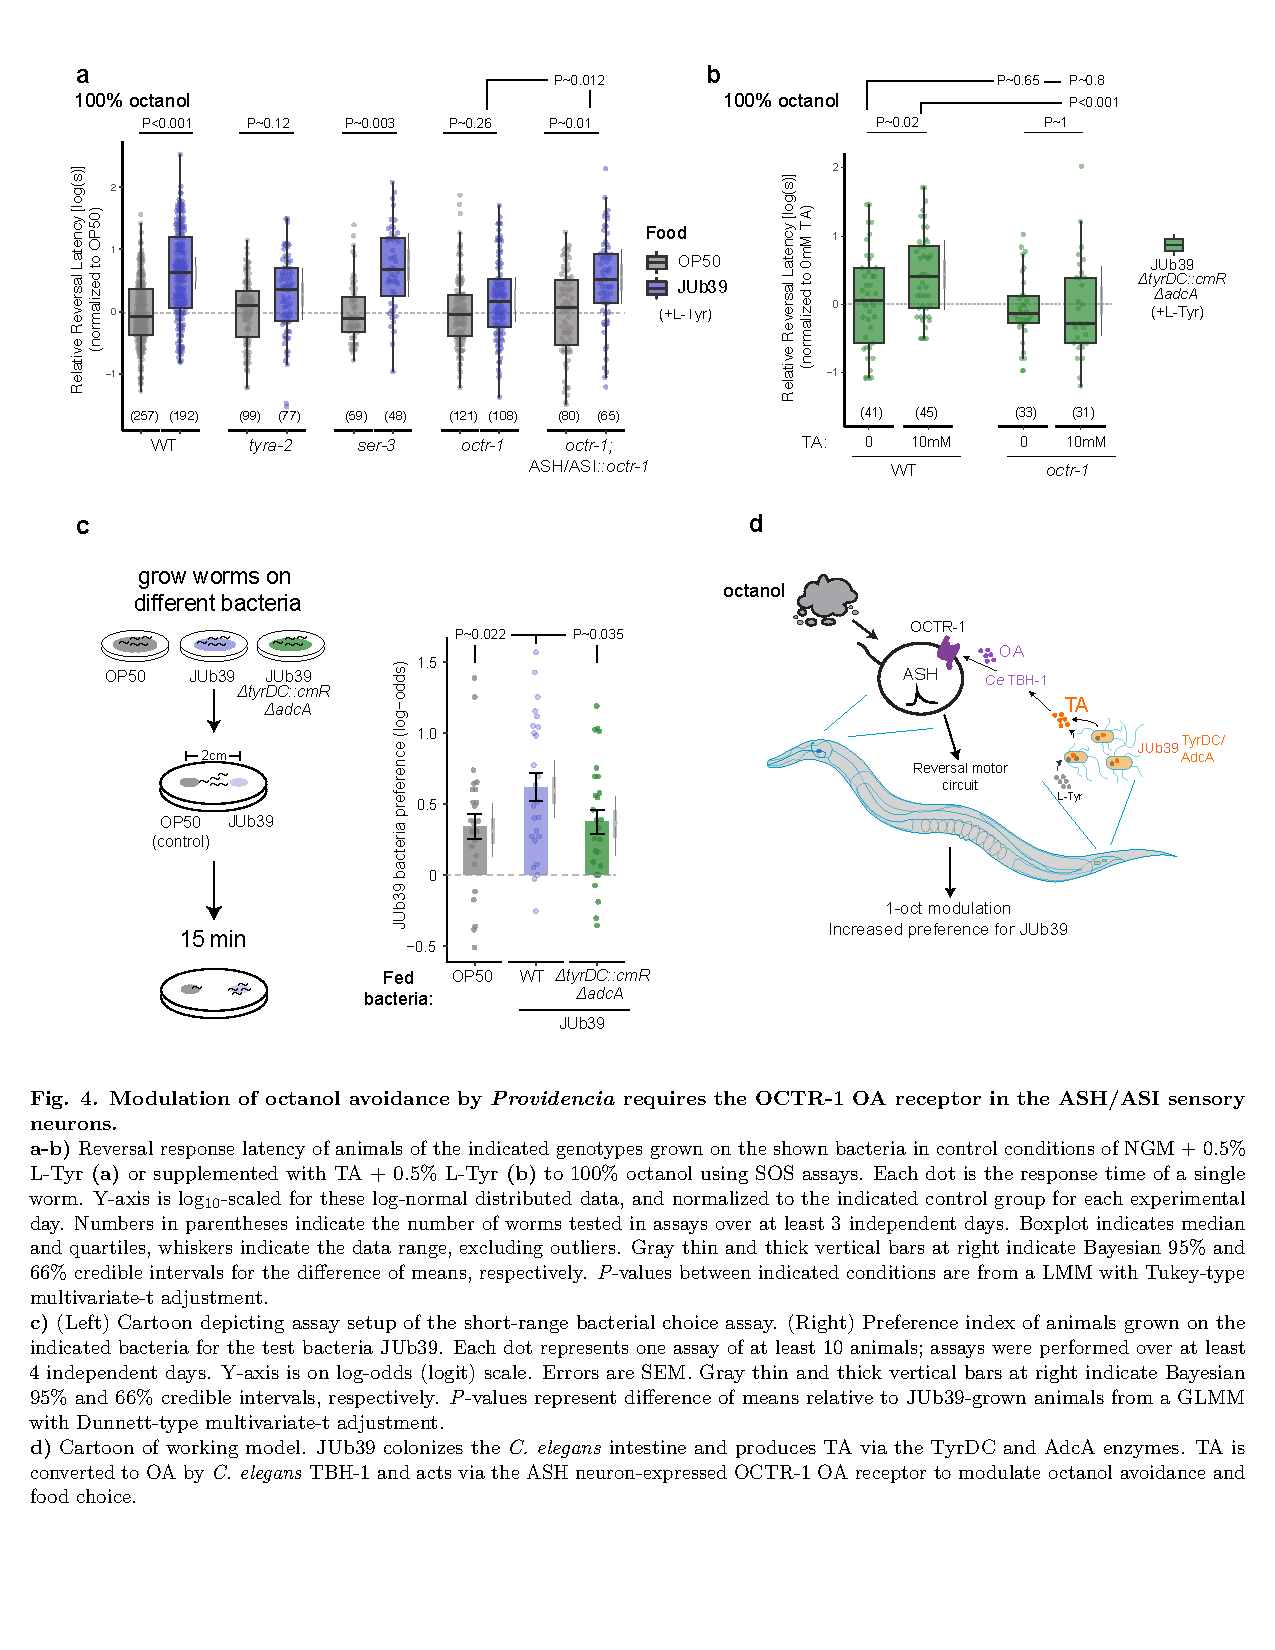
\includegraphics[width=1.05\linewidth]{Figure4} \end{center}

\vskip 0.2in \vskip 0.2in

\begin{center}
\textbf{Methods}
\end{center}

\noindent \textbf{Strains}

\emph{C. elegans}: All \emph{C. elegans} strains were maintained on
nematode growth medium (NGM) at 20ºC. \emph{sra-6p::octr-1} plasmid
(pMOD100) was injected at 10 ng/\(\mu\)l together with the
\emph{unc-122p::gfp} coinjection marker at 30 ng/\(\mu\)l to generate
transgenic strains. Two independent lines were examined for
\emph{octr-1} rescue experiments.

\emph{Bacteria}: For all experiments, bacterial strains were streaked
from glycerol stocks prior to use and grown to saturation in LB media at
37ºC. For conditioned media, bacteria were grown to saturation in NGM
media overnight at 37ºC, then cleared by centrifugation at 14,000g for 3
minutes. Prior to use, conditioned media or NGM was supplemented with 5x
concentrated OP50 from a saturated LB culture to prevent starvation. To
expose animals to bacterial odors, worms were grown on seeded NGM plates
whose lids were replaced with NGM plates containing the test bacteria;
these were sealed with parafilm. For L-Tyr and TA supplementation
experiments, 0.5\% L-Tyr (Sigma T3754) or 4mM or 10mM TA (Sigma T2879)
were added to the NGM media and agar prior to pouring plates. Plasmids
were transformed into JUb39 and OP50 via electroporation. Deletions in
JUb39 were induced using homologous recombination with the
temperature-sensitive pSC101 replicon at 42ºC, and \emph{sacB}-sucrose
counter-selection at 30ºC, in the absence of NaCl as
described\textsuperscript{41}, with the exception that bacteria were
incubated for 1 hour at room temperature in the presence of 10mM
arabinose for lambda Red induction prior to selection at 42ºC. Deletions
were confirmed by sucrose resistance and kanamycin sensitivity, followed
by PCR and sequencing of deleted intervals.

\vspace{2\parsep}

\noindent   \textbf{Molecular biology}

The \emph{octr-1} cDNA was a gift from Dr.~Richard Komuniecki. The cDNA
was amplified by PCR and cloned using Gibson homology cloning. The 3.8kb
\emph{sra-6} promoter sequence was cloned from genomic DNA. Vector maps
are available on Github
(\url{https://github.com/SenguptaLab/ProvidenciaChemo.git}). For
introduction of deletions via homologous recombination in JUb39,
pKD46-derivative plasmids containing a lambda Red cassette and deletion
homology arms for JUb39 \textit{tyrDC} and \textit{adcA} were
constructed (denoted pMOD102 and pMOD107, respectively). Briefly, the
\emph{cas9} coding region and sgRNA regions of pDK46-derivative
pCAS\textsuperscript{42} were deleted and replaced with the \emph{sacB}
sequence from pCM433\textsuperscript{43} via PCR and Gibson homology
cloning. For pMOD102, 5' and 3' homology arms were approximately 400bp
each flanking a 1233bp deletion of the \textit{tyrDC} coding sequence
which was replaced with a chloramphenicol resistance cassette. For
pMOD107, 5' and 3' homology arms were 701 and 422bp, respectively,
flanking a 1398bp deletion of the \textit{adcA} CDS. For expression of
mCherry in OP50 and JUb39, a pUCP20T-mCherry plasmid\textsuperscript{44}
was modified to replace \emph{bla}(ampR) with \emph{aph}(kanR).

\vspace{2\parsep}

\noindent   \textbf{Microscopy}

All fluorescence microscopy was performed using animals anesthetized
with 100 mM levamisole (Sigma Aldrich). Animals were imaged on 2\%
agarose pads using an upright Zeiss Axio Imager with a 63X oil immersion
objective.

\emph{Quantification of intestinal bacterial cell numbers:} All
rod-shaped punctae in the intestines of young adult worms of
approximately 1-2\(\mu\)m were included in the quantification. Each
animal was recorded in one of three categories containing 0,
\textless{}10, or \textgreater{}10 cells per animal. Exact numbers in
animals bearing over 10 cells were not recorded, but rarely exceeded
approximately 100 cells.

\emph{Fluorescence intensity measurements:} All images were collected in
z-stacks of 0.5 \(\mu\)m through the heads of young adult worms.
Quantification was performed using ImageJ (NIH). Fluorescence was
quantified by identifying the focal plane in which the cell soma was
visible, followed by manually drawing an ROI around the soma. Mean pixel
intensity was recorded for each neuron pair per animal and the average
of fluorescence in each animal is shown.

\vspace{2\parsep}

\noindent \textbf{Behavioral assays}

\emph{Long-range chemotaxis}: Long-range chemotaxis assays were
performed essentially as described\textsuperscript{7,45}. Worms were
cultured for 1 generation with the relevant bacteria prior to the assay.
Assays were performed using 10cm square NGM plates. The number of worms
in two horizontal rows adjacent to the odor and ethanol spots were
quantified.

\emph{SOS assays:} Smell-on-a-stick (SOS) assays in response to
1-octanol or 2-nonanone were performed as
described\textsuperscript{9,26}. NGM plates were pre-dried for 1 hour
prior to assays. Age-matched young adult animals were picked from food
to a clean transfer plate and allowed to briefly crawl away from food
for approximately 1 min. Animals were then transferred to another clean
NGM plate for 15 minutes prior to assaying responses to 100\% octanol
(Sigma O4500) and 100\% 2-nonanone (Sigma 108731), or 20 minutes for
30\% octanol assays. 30\% octanol was prepared immediately before the
assay by dilution in 200-proof ethanol (Acros Organics 61509-0010).

\emph{Short-range bacterial choice assay:} Animals were raised and
prepared identically to those used in long-range chemotaxis assays, with
the exception that the final wash with water was omitted. NGM plates
containing 2 15\(\mu\)L spots of overnight-grown bacterial food
concentrated to OD600 \textasciitilde{} 10 placed 2cm apart were allowed
to dry, then incubated with a closed lid for 5 hrs at room temperature.
Approximately 30 animals were placed between the two spots, and excess
liquid was removed. Animals were allowed to navigate for 15 minutes
following which 2\(\mu\)L of sodium azide was applied to each spot to
anesthetize worms. Very little lawn-leaving behavior was observed during
this short time period. Adult animals on the control spot and test spot
were counted.

\emph{Osmotic avoidance assay:} Animals off the bacterial food on the
cultivation plate were picked using a 10\% methyl cellulose polymer
solution and placed in the center of an NGM plate with a ring of 8M
glycerol containing bromophenol blue (Sigma B0126). The number of worms
inside and outside of the ring were counted after 10 mins.

\vspace{2\parsep}

\noindent   \textbf{Bacteria genome sequencing}

Sequencing was performed by the Broad Technology Labs at the Broad
Institute. Resulting PacBio reads for JUb39 and PYb007 were assembled
using Canu\textsuperscript{46} v1.8
(\url{https://github.com/marbl/canu.git}). Assemblies were trimmed,
oriented and circularized using Circlator\textsuperscript{47} v1.5.5
(\url{https://sanger-pathogens.github.io/circlator/}).

\vspace{2\parsep}

\noindent \textbf{Phylogenetic analysis of group II pyridoxal-dependent
decarboxylase genes}

JUb39 TyrDC and AdcA were initially identified as the only significant
hits via a tblastn search of the draft JUb39 genome assembly using
\emph{Enterococcus faecalis} TyrDC as a query sequence. An initial
BLASTP screen of the nr sequence database restricted to bacteria was
performed using the \emph{P. alcalifaciens} JUb39 TyrDC and AdcA coding
regions. Searches were performed hierarchically, limited initially to
\emph{Enterobacteriaceae}, followed by \emph{Enterobacterales,
Gammaproteobacteria, Proteobacteria} and finally all \emph{Eubacteria}.
With the exception of members of \emph{Morganellaceae}
(\emph{Providencia, Proteus, Morganella, Xenorhabdus, Photorhabdus,
Arsenophonus} and \emph{Moellerella}), only two protein sequences per
genus were retained for subsequent phylogenetic analysis. Representative
group II decarboxylase enzymes with known substrate specificity from
\emph{Eukaryota} and \emph{Archaea} as well as glutamate decarboxylase
(GadA/B) and histidine decarboxylase sequences were also included.

Multiple sequence alignments were produced using the Phylomizer workflow
(\url{https://github.com/Gabaldonlab/phylomizer}), which used the
MUSCLE\textsuperscript{48} v3.8.31 (\url{http://www.drive5.com/muscle}),
MAFFT\textsuperscript{49} v7.407
(\url{https://mafft.cbrc.jp/alignment/software}) and
Kalign\textsuperscript{50} v2.04
(\url{http://msa.sbc.su.se/cgi-bin/msa.cgi}) multiple sequence aligners;
these were trimmed to produce a consensus alignment using
trimAL\textsuperscript{51} v1.4rev15
(\url{https://github.com/scapella/trimal}). An initial phylogenetic tree
was produced using PhyML\textsuperscript{52} v3.3.20180621
(\url{http://www.atgc-montpellier.fr/phyml/}) using the NNI algorithm
with an LG substitution model. This tree showed three major,
well-supported clusters containing: (1) \emph{Enterococcus} and
\textit{Providencia} TyrDCs - denoted ``\emph{Enterococcus}-type TDC'',
(2) Eukaryotic AADCs denoted ``Eukaryotic-type AADC'', and (3)
\emph{Morganella} AdcA and \textit{Providencia} AdcA.

Based on this initial tree, a second tblastn search was used to
determine the presence or absence of homologous genes among complete
\emph{Gammaproteobacteria} genomes. \emph{Enterococcus faecalis} TyrDC
and \textit{C. elegans} TDC-1 were used as tblastn search query
sequences. Hierarchical search was performed as described above, limited
to an e-value cutoff of 10-5. A maximum of 2 highly similar sequences
were retained per genus for phylogenetic analysis as listed in Table S1.

A final phylogenetic tree was constructed using the amino acid sequences
derived from these tblastn queries. These were assembled into a
consensus alignment using the Phylomizer workflow as described above.
ProtTest\textsuperscript{53}
(\url{https://github.com/ddarriba/prottest3}) was used to identify the
optimal model for likelihood estimation, using Aikake Information
Criterion (AIC) values for selection. The model selected and subject to
PhyML analysis was an LG model with discrete gamma distribution, an
estimated proportion of invariant sites (+I), empirical frequencies of
amino acids (+F), estimated gamma shape parameter (+G) for rate
variation among sites with the default 4 substitution rate categories,
and the subtree pruning and regrafting (SPR) algorithm. 100 bootstrap
pseudoreplicates were analyzed. Representatives from the resulting
phylogeny were used to categorize and compile the cladogram in Fig.
3b-c. Adjacent genomic sequences, up to 3 CDS 5' or 3', were examined
for genes encoding amino-acid permeases or transporters in an apparent
operon as defined by close proximity and same orientation with respect
to each tblastn hit (Table S1).

\vspace{2\parsep}

\noindent \textbf{Molecular modeling}

The putative amino acid sequence for JUb39 TyrDC was used to model
active site residues using the \emph{Lb}-TyrDC crystal structure in
complex with PLP (5hsj.1\textsuperscript{34}) as a template guide using
SWISS-MODEL (\url{https://swissmodel.expasy.org}). This resulted in a
Qmean Z-score of 0.33, indicative of good agreement between structures.
This process was also attempted with AdcA, and modeling was performed
with the top 6 available structures based on sequence homology. The
maximum QMean of AdcA was found with \emph{Lb}-TyrDC, but with a value
-5.71, indicative of low quality. Resulting models were visualized using
Chimera\textsuperscript{54} v1.13.1
(\url{https://www.cgl.ucsf.edu/chimera/}). For Fig. 3d, L-Tyrosine was
manually docked according to the reported docking
position\textsuperscript{34} for illustrative purposes only.

\vspace{2\parsep}

\noindent \textbf{Statistical analyses}

All statistical analyses were performed in R
(\url{https://www.R-project.org/}) and RStudio
(\url{http://www.rstudio.com}). For modulation index and relative
latency figures, data were were normalized to the relevant control group
mean value for each experimental day on the log scale via subtraction.
Outliers in boxplots were defined as greater than 1.5*interquartile
range, but were included for analysis. All statistical analyses were
performed on raw, non-normalized data. To avoid inflated \emph{P}-values
and account for non-independence of observations, we employed
mixed-effects regression analysis in lieu of simple ANOVA and t-tests.
For behavioral assays, frequentist statistical comparisons were
performed using a binomial generalized linear mixed-effects model (GLMM)
with a logit link function for chemotaxis and food choice assays, while
a linear mixed-effects model (LMM) on log\textsubscript{10}-transformed
data was used to analyze SOS assays using the `lme4' package. In all
cases, a random intercept term for assay plate was used to account for
non-independence of animals on each assay plate and random intercept for
date was used to account for day-to-day variability. In the presence of
interactions, for example the effects of bacterial strains across
different odorants in Fig. 1a, a random slope term per date was also
used when appropriate. Estimated \emph{P}-values for pairwise comparison
of fixed effects were determined using Kenward-Roger approximated
degrees of freedom as implemented in the `emmeans' and `pbkrtest'
packages. In nearly all cases, inclusion of random effects model terms
resulted in conservative \emph{P}-value estimates compared to a simple
ANOVA. In the event of singular model fit, any random slope term,
followed by random date effect terms were removed to allow convergence.
For Wald statistics of model terms, packages `lmerTest' or `car' were
used.

Additionally, for each dataset, a maximal Bayesian model was fit using
the `rstanarm' and `rstan' packages. Data presented are posterior
credible intervals for fixed effect levels derived from posterior fitted
values of the MCMC chains as implemented by the `emmeans', `coda',
`bayesplot' and `tidybayes' packages. Post-hoc corrections for multiple
comparisons and type-I error were implemented using the `emmeans'
package. For comparison of intestinal bacterial cell numbers, an ordinal
logistic regression was performed using the `MASS' package and `polr'
function. Categories of cell numbers were considered ordered factors of
`none', `some' or `many' cells.

\vspace{2\parsep}

\noindent \textbf{Sample preparation for HPLC-MS}

Approximately 10,000 mixed-staged worms in 1.5mL microfuge tubes were
lyophilized for 18-24 hrs using a VirTis BenchTop 4K Freeze Dryer. After
the addition of two stainless steel grinding balls and 1mL of 80\%
methanol, samples were sonicated for 5 min (2 sec on/off pulse cycle at
90 A) using a Qsonica Q700 Ultrasonic Processor with a water bath cup
horn adaptor (Model 431C2). Following sonication, microfuge tubes were
centrifuged at 10,000 RCF for 5 min in an Eppendorf 5417R centrifuge.
800\(\mu\)L of the resulting supernatant was transferred to a clean 4mL
glass vial, and 800\(\mu\)L of fresh methanol added to the sample. The
sample was sonicated and centrifuged as described, and the resulting
supernatant was transferred to the same receiver vial and concentrated
to dryness in an SC250EXP Speedvac Concentrator coupled to an RVT5105
Refrigerated Vapor Trap (Thermo Scientific). The resulting powder was
suspended in 120\(\mu\)L of 100\% methanol, followed by vigorous vortex
and brief sonication. This solution was transferred to a clean microfuge
tube and subjected to centrifugation at 20,000 RCF for 10 min in an
Eppendorf 5417R centrifuge to remove precipitate. The resulting
supernatant was transferred to an HPLC vial and analyzed by HPLC-MS.

\vspace{2\parsep}

\noindent \textbf{HPLC-MS analyses}

Reversed-phase chromatography was performed using a Vanquish LC system
controlled by Chromeoleon Software (ThermoFisher Scientific) and coupled
to an Orbitrap Q-Exactive High Field mass spectrometer controlled by
Xcalibur software (ThermoFisher Scientific). Methanolic extracts
prepared as described above were separated on an Agilent Zorbax Eclipse
XDB-C18 column (150 mm x 2.1 mm, particle size 1.8 \(\mu\)m) maintained
at 40°C with a flow rate of 0.5mL/min. Solvent A: 0.1\% formic acid in
water; solvent B: 0.1\% formic acid in acetonitrile (ACN). A/B gradient
started at 5\% B for 3 min after injection and increased linearly to
98\% B at 20 min, holding at 98\% B until 25 min, followed by a 0.1 min
gradient to 5\% B, held until 28 min. Mass Spectrometer parameters:
spray voltage 3.0 kV, capillary temperature 380°C, probe heater
temperature 400°C; sheath, auxiliary, and sweep gas 60, 20, and 1 AU,
respectively. S-Lens RF level: 50, resolution 240,000 at m/z 200, AGC
target 3E6, maximum injection time (IT) 500 msec. Each sample was
analyzed in negative and positive electrospray ionization modes with m/z
range 150--800. Parameters for MS/MS (dd-MS2): MS1 resolution: 60,000,
AGC Target: 3E6, max IT 100 msec. MS2 resolution: 30,000, AGC Target:
1E5, max IT 50 msec. Isolation window 1.0 m/z, stepped normalized
collision energy (NCE) 10, 30; dynamic exclusion: 5 sec.~Top 10 masses
selected for MS/MS per scan. LC-MS data were analyzed via manual
integration in Excalibur (ThermoFisher Scientific).

\vspace{2\parsep}

\noindent \textbf{Data availability}

All statistical analysis code and raw data necessary to reproduce these
analyses are available
{[}\url{https://github.com/SenguptaLab/ProvidenciaChemo.git}{]}. Draft
genome assemblies will be deposited in Genbank.

\vspace{2\parsep}

\begin{center}
\textbf{Acknowledgements}
\end{center}

\noindent We thank Richard Komuniecki for the \emph{octr-1} cDNA,
multiple members of the \emph{C. elegans} community for bacterial
strains (listed in Table S2), and the \emph{Caenorhabditis} Genetics
Center for \emph{C. elegans} strains. We are grateful to the Broad
Technology Labs for bacterial genome sequencing. We thank Sue Lovett,
Laura Laranjo and the Sengupta lab for advice. We acknowledge the
Sengupta lab and Cori Bargmann for comments on the manuscript. This work
was partly supported by the NIH (T32 NS007292 and F32 DC013711 -- M.O'D,
R01 GM088290 and R35 GM131877 -- F.C.S., and R35 GM122463 and R21
NS101702 -- P.S.), and the NSF (IOS 1655118 -- P.S.).

\vspace{2\parsep}

\begin{center}
\textbf{References}
\end{center}

\noindent

\begin{enumerate}
\def\labelenumi{\arabic{enumi}.}
\tightlist
\item
  Douglas, A. E. \emph{Fundamentals of Microbiome Science: How Microbes
  Shape Animal Biology.} (Princeton University Press, 2018).
\item
  Strandwitz, P. Neurotransmitter modulation by the gut microbiota.
  \emph{Brain Research} \textbf{1693}, 128--133 (2018).
\item
  Zhang, J., Holdorf, A. D. \& Walhout, A. J. \emph{C. elegans} and its
  bacterial diet as a model for systems-level understanding of
  host-microbiota interactions. \emph{Curr. Opin. Biotechnol.}
  \textbf{46}, 74--80 (2017).
\item
  Schulenburg, H. \& Félix, M.-A. The natural biotic environment of
  \emph{Caenorhabditis elegans}. \emph{Genetics} \textbf{206}, 55--86
  (2017).
\item
  Meisel, J. D. \& Kim, D. H. Behavioral avoidance of pathogenic
  bacteria by \emph{Caenorhabditis elegans}. \emph{Trends Immunol.}
  \textbf{35}, 465--470 (2014).
\item
  Samuel, B. S., Rowedder, H., Braendle, C., Félix, M.-A. \& Ruvkun, G.
  \emph{Caenorhabditis elegans} responses to bacteria from its natural
  habitats. \emph{Proc. Natl. Acad. Sci. USA} \textbf{113}, E3941--9
  (2016).
\item
  Bargmann, C. I., Hartwieg, E. \& Horvitz, H. R. Odorant-selective
  genes and neurons mediate olfaction in \emph{C. elegans}. \emph{Cell}.
  \textbf{74}, 515--527 (1993).
\item
  Song, B.-M., Faumont, S., Lockery, S. \& Avery, L. Recognition of
  familiar food activates feeding via an endocrine serotonin signal in
  \emph{Caenorhabditis elegans}. \emph{Elife} \textbf{2}, e00329 (2013).
\item
  Chao, M. Y., Komatsu, H., Fukuto, H. S., Dionne, H. M. \& Hart, A. C.
  Feeding status and serotonin rapidly and reversibly modulate a
  \emph{Caenorhabditis elegans} chemosensory circuit. \emph{Proc. Natl.
  Acad. Sci. USA} \textbf{101}, 15512--15517 (2004).
\item
  Liang, B., Moussaif, M., Kuan, C.-J., Gargus, J. J. \& Sze, J. Y.
  Serotonin targets the DAF-16/FOXO signaling pathway to modulate stress
  responses. \emph{Cell Metab.} \textbf{4}, 429--440 (2006).
\item
  Entchev, E. V. et al.~A gene-expression-based neural code for food
  abundance that modulates lifespan. \emph{Elife} \textbf{4}, e06259
  (2015).
\item
  Avery, L. \& Shtonda, B. B. Food transport in the \emph{C. elegans}
  pharynx. \emph{J. Exp. Biol.} \textbf{206}, 2441--2457 (2003).
\item
  Avery, L. The genetics of feeding in \emph{Caenorhabditis elegans}.
  \emph{Genetics} \textbf{133}, 897--917 (1993).
\item
  Berg, M. et al.~Assembly of the \emph{Caenorhabditis elegans} gut
  microbiota from diverse soil microbial environments. \emph{ISME J}
  (2016). \url{doi:10.1038/ismej.2015.253}
\item
  Dirksen, P. et al.~The native microbiome of the nematode
  \emph{Caenorhabditis elegans}: gateway to a new host-microbiome model.
  \emph{BMC Biol}. \textbf{14}, 38 (2016).
\item
  Tan, M.-W., Mahajan-Miklos, S. \& Ausubel, F. M. Killing of
  \emph{Caenorhabditis elegans} by \emph{Pseudomonas aeruginosa} used to
  model mammalian bacterial pathogenesis. \emph{Proc. Natl. Acad. Sci.
  USA} \textbf{96}, 715--720 (1999).
\item
  Irazoqui, J. E. et al.~Distinct pathogenesis and host responses during
  infection of \emph{C. elegans} by \emph{P. aeruginosa} and \emph{S.
  aureus}. \emph{PLoS Pathog.} \textbf{6}, e1000982 (2010).
\item
  Wragg, R. T. et al.~Tyramine and octopamine independently inhibit
  serotonin-stimulated aversive behaviors in \emph{Caenorhabditis
  elegans} through two novel amine receptors. \emph{J Neurosci.}
  \textbf{27}, 13402--13412 (2007).
\item
  Mills, H. et al.~Monoamines and neuropeptides interact to inhibit
  aversive behaviour in \emph{Caenorhabditis elegans}. \emph{EMBO J.}
  \textbf{31}, 667--678 (2012).
\item
  Harris, G. P. et al.~The monoaminergic modulation of sensory-mediated
  aversive responses in \emph{Caenorhabditis elegans} requires
  glutamatergic/peptidergic cotransmission. \emph{J. Neurosci.}
  \textbf{30}, 7889--7899 (2010).
\item
  Ezak, M. J. \& Ferkey, D. M. The \emph{C. elegans} D2-Like dopamine
  receptor DOP-3 decreases behavioral sensitivity to the olfactory
  stimulus 1-octanol. \emph{PLoS ONE} \textbf{5}, e9487 (2010).
\item
  Ezcurra, M., Tanizawa, Y., Swoboda, P. \& Schafer, W. R. Food
  sensitizes \emph{C. elegans} avoidance behaviours through acute
  dopamine signalling. \emph{EMBO J.} \textbf{30}, 1110--1122 (2011).
\item
  Alkema, M. J., Hunter-Ensor, M., Ringstad, N. \& Horvitz, H. R.
  Tyramine functions independently of octopamine in the
  \emph{Caenorhabditis elegans} nervous system. \emph{Neuron}
  \textbf{46}, 247--260 (2005).
\item
  Lints, R. \& Emmons, S. W. Patterning of dopaminergic neurotransmitter
  identity among \emph{Caenorhabditis elegans} ray sensory neurons by a
  TGFbeta family signaling pathway and a Hox gene. \emph{Development}
  \textbf{126}, 5819--5831 (1999).
\item
  Sze, J. Y., Victor, M., Loer, C., Shi, Y. \& Ruvkun, G. Food and
  metabolic signalling defects in a \emph{Caenorhabditis elegans}
  serotonin-synthesis mutant. \emph{Nature} \textbf{403}, 560--564
  (2000).
\item
  Troemel, E. R., Chou, J. H., Dwyer, N. D., Colbert, H. A. \& Bargmann,
  C. I. Divergent seven transmembrane receptors are candidate
  chemosensory receptors in \emph{C. elegans}. \emph{Cell} \textbf{83},
  207--218 (1995).
\item
  Artyukhin, A. B. et al.~Succinylated octopamine ascarosides and a new
  pathway of biogenic amine metabolism in \emph{Caenorhabditis elegans}.
  \emph{J. Biol. Chem.} \textbf{288}, 18778--18783 (2013).
\item
  Pugin, B. et al.~A wide diversity of bacteria from the human gut
  produces and degrades biogenic amines. \emph{Microb. Ecol. Health
  Dis.} \textbf{28}, 1353881 (2017).
\item
  Barbieri, F., Montanari, C., Gardini, F. \& Tabanelli, G. Biogenic
  Amine Production by Lactic Acid Bacteria: A Review. \emph{Food}
  \textbf{8}, 17 (2019).
\item
  Marcobal, Á., Martín-Álvarez, P. J., Moreno-Arribas, M. V. \& Muñoz,
  R. A multifactorial design for studying factors influencing growth and
  tyramine production of the lactic acid bacteria \emph{Lactobacillus
  brevis} CECT 4669 and \emph{Enterococcus faecium} BIFI-58. \emph{Res.
  Microbiol.} \textbf{157}, 417--424 (2006).
\item
  Sandmeier, E., Hale, T. I. \& Christen, P. Multiple evolutionary
  origin of pyridoxal-5'-phosphate-dependent amino acid decarboxylases.
  \emph{Eur. J. Biochem.} \textbf{221}, 997--1002 (1994).
\item
  Connil, N. et al.~Identification of the \emph{Enterococcus faecalis}
  Tyrosine decarboxylase operon involved in tyramine production.
  \emph{Appl. Environ. Microb.} \textbf{68}, 3537--3544 (2002).
\item
  Linares, D. M., Fernández, M., Martín, M. C. \& Alvarez, M. A.
  Tyramine biosynthesis in \emph{Enterococcus durans} is
  transcriptionally regulated by the extracellular pH and tyrosine
  concentration. \emph{Microb. Biotechnol.} \textbf{2}, 625--633 (2009).
\item
  Zhu, H. et al.~Crystal structure of tyrosine decarboxylase and
  identification of key residues involved in conformational swing and
  substrate binding. \emph{Sci. Rep.} \textbf{6}, 27779 (2016).
\item
  Rex, E. et al.~TYRA-2 (F01E11.5): a \emph{Caenorhabditis elegans}
  tyramine receptor expressed in the MC and NSM pharyngeal neurons.
  \emph{J. Neurochem.} \textbf{94}, 181--191 (2005).
\item
  Chute, C. D. et al.~Co-option of neurotransmitter signaling for
  inter-organismal communication in \emph{C. elegans}. \emph{Nat.
  Commun.} \textbf{10}, 3186 (2019).
\item
  Elgaali, H. et al.~Comparison of long-chain alcohols and other
  volatile compounds emitted from food-borne and related Gram positive
  and Gram negative bacteria. \emph{J. Basic Microbiol.} \textbf{42},
  373--380 (2002).
\item
  Worthy, S. E. et al.~Identification of attractive odorants released by
  preferred bacterial food found in the natural habitats of \emph{C.
  elegans}. \emph{PLoS ONE} \textbf{13}, e0201158 (2018).
\item
  Yoshida, K. et al.~Odour concentration-dependent olfactory preference
  change in \emph{C. elegans}. \emph{Nat. Commun.} \textbf{3}, 739
  (2012).
\item
  Zhang, F. et al. \emph{Caenorhabditis elegans} as a model for
  microbiome research. \emph{Front. Microbiol.} \textbf{8}, 485 (2017).
\item
  Blomfield, I. C., Vaughn, V., Rest, R. F. \& Eisenstein, B. I. Allelic
  exchange in \emph{Escherichia coli} using the \emph{Bacillus subtilis
  sacB} gene and a temperature-sensitive pSC101 replicon. \emph{Mol.
  Microbiol.} \textbf{5}, 1447--1457 (1991).
\item
  Jiang, Y. et al.~Multigene editing in the \emph{Escherichia coli}
  genome via the CRISPR-Cas9 system. \emph{Appl. Environ. Microb.}
  \textbf{81}, 2506--2514 (2015).
\item
  Marx, C. J. Development of a broad-host-range sacB-based vector for
  unmarked allelic exchange. \emph{BMC Res. Notes} \textbf{1}, 1 (2008).
\item
  Barbier, M. \& Damron, F. H. Rainbow Vectors for broad-range bacterial
  fluorescence labeling. \emph{PLoS ONE} \textbf{11}, e0146827 (2016).
\item
  Troemel, E. R., Kimmel, B. E. \& Bargmann, C. I. Reprogramming
  chemotaxis responses: sensory neurons define olfactory preferences in
  \emph{C. elegans}. \emph{Cell} \textbf{91}, 161--169 (1997).
\item
  Koren, S. et al.~Canu: scalable and accurate long-read assembly via
  adaptive k-mer weighting and repeat separation. \emph{Genome Res.}
  \textbf{27}, 722--736 (2017).
\item
  Hunt, M. et al.~Circlator: automated circularization of genome
  assemblies using long sequencing reads. \emph{Genome Biol}.
  \textbf{16}, 294--10 (2015).
\item
  Edgar, R. C. MUSCLE: multiple sequence alignment with high accuracy
  and high throughput. \emph{Nucleic Acids Res.} \textbf{32}, 1792--1797
  (2004).
\item
  Katoh, K. \& Standley, D. M. MAFFT multiple sequence alignment
  software version 7: improvements in performance and usability.
  \emph{Mol. Biol. Evol.} \textbf{30}, 772--780 (2013).
\item
  Lassmann, T. \& Sonnhammer, E. L. L. Kalign--an accurate and fast
  multiple sequence alignment algorithm. \emph{BMC Bioinformatics}
  \textbf{6}, 298--9 (2005).
\item
  Capella-Gutiérrez, S., Silla-Martínez, J. M. \& Gabaldón, T. trimAl: a
  tool for automated alignment trimming in large-scale phylogenetic
  analyses. \emph{Bioinformatics} \textbf{25}, 1972--1973 (2009).
\item
  Guindon, S. \& Gascuel, O. A simple, fast, and accurate algorithm to
  estimate large phylogenies by maximum likelihood. \emph{Syst. Biol.}
  \textbf{52}, 696--704 (2003).
\item
  Darriba, D., Taboada, G. L., Doallo, R. \& Posada, D. ProtTest 3: fast
  selection of best-fit models of protein evolution.
  \emph{Bioinformatics} \textbf{27}, 1164--1165 (2011).
\item
  Pettersen, E. F. et al.~UCSF Chimera--a visualization system for
  exploratory research and analysis. \emph{J Comput. Chem.} \textbf{25},
  1605--1612 (2004).
\end{enumerate}


\end{document}
